\subsection{Patrones de diseño}

En el desarrollo de software, los patrones de diseño son soluciones probadas y reutilizables para problemas comunes que los desarrolladores enfrentan al diseñar aplicaciones.

\textbf{Patrón de Convención sobre Configuración (CoC)}

El sistema adopta el Patrón CoC, que permite gestionar configuraciones a través de archivos externos. Esta práctica facilita la personalización y la flexibilidad, permitiendo ajustes sin necesidad de modificar el código fuente. Esto es crucial para adaptar la aplicación a diferentes entornos y necesidades organizacionales, mejorando la mantenibilidad y escalabilidad del sistema.

En la implementación del Patrón de CoC, se establecieron valores predeterminados para la configuración LDAP y otros aspectos. Se implementó soporte para archivos de configuración en formato JSON y YAML, validados mediante JSON Schema, para permitir ajustes específicos. Esta aproximación no solo facilita la configuración inicial de la aplicación, sino que también ofrece flexibilidad para personalizar la configuración según los requisitos del usuario final.

\textbf{Patrón de Observador}
El Patrón Observador es una técnica de diseño fundamental en el desarrollo de software para establecer relaciones de dependencia. En este patrón, cuando un objeto cambia su estado, todos los objetos dependientes son notificados y actualizados automáticamente.

En el contexto de SvelteKit, el patrón Observador es crucial para la gestión de la reactividad a través de los stores. En la \autoref{fig:loader-store-reaction} se muestra un componente que solo es visible si el valor de la store \textbf{loading} de la \autoref{fig:loader-store-declaration} tiene valor \textbf{true}. Por lo tanto cualquier componente que se modifique el valor de esta store provoca una mutación en el estado del componente de la \autoref{fig:loader-store-reaction}.

\begin{figure}[h]
    \centering
    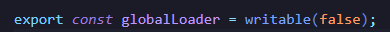
\includegraphics[width=\linewidth]{images/code/loader-store-declaration.png}
    \caption{Declaracion de un store en Sveltekit}
    \label{fig:loader-store-declaration}
\end{figure}

\begin{figure}[h]
    \centering
    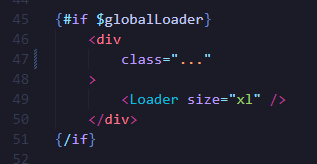
\includegraphics{images/code/loader-store-reaction.png}
    \caption{Reacción al cambio en la store}
    \label{fig:loader-store-reaction}
\end{figure}

\textbf{Patrón inyeccion de dependencias}

El patrón de Inyección de Dependencias es un patrón de diseño que busca mejorar la modularidad y la reutilización del código al desacoplar la creación de objetos de su uso. En lugar de que una clase o módulo cree directamente sus dependencias, estas son proporcionadas desde el exterior.

La \textit{Context API}(API de contexto) de Svelte es una herramienta que facilita la comunicación entre componentes sin necesidad de pasar propiedades a través de cada nivel del árbol de componentes. Este mecanismo se utiliza para compartir datos y servicios globales dentro de una aplicación, lo que permite una gestión más eficiente de las dependencias y contribuye a un diseño más limpio y modular.

En el contexto del sistema, la API de contexto se utiliza para inyectar la configuración de la aplicación relacionada con la página actual (\autoref{fig:context-api-dep-injection}). Esto permite que los componentes accedan a la configuración específica de la página sin necesidad de recibirla a través de props (\autoref{fig:context-api-usage}).

\begin{figure}[h]
    \centering
    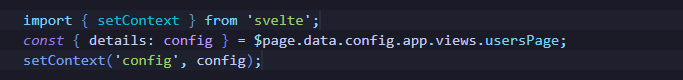
\includegraphics[width=\linewidth]{images/code/context-api-dep-injection.png}
    \caption{Uso de la API de Contexto de Sveltekit para inyectar la configuración de la página}
    \label{fig:context-api-dep-injection}
\end{figure}

\begin{figure}[h]
    \centering
    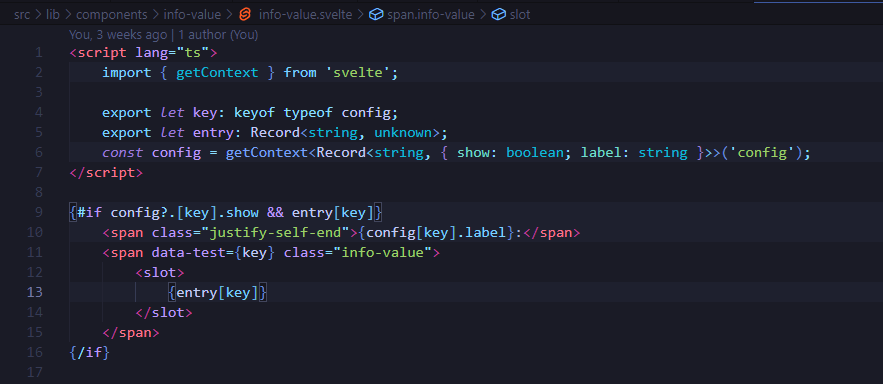
\includegraphics[width=\linewidth]{images/code/context-api-usage.png}
    \caption{Uso de la API de Contexto de Sveltekit para leer la configuracion de la página}
    \label{fig:context-api-usage}
\end{figure}